\documentclass{article}
\usepackage{tikz}
\usepackage{amsmath}

\usetikzlibrary{shapes.geometric, arrows}

\tikzstyle{startstop} = [rectangle, rounded corners, minimum width=3cm, 
  minimum height=1cm,text centered, draw=black, fill=red!30]

\tikzstyle{io} = [rectangle, rounded corners, 
  trapezium right angle=110, minimum width=2cm, minimum height=0.8cm, 
  text centered, draw=black, fill=blue!30]

\tikzstyle{process} = [rectangle, minimum width=3cm, minimum
  height=1cm, text centered, draw=black, fill=orange!30]

\tikzstyle{decision} = [diamond, minimum width=3cm, minimum
  height=1cm, text centered, draw=black, fill=green!30]

\tikzstyle{arrow} = [thick,->,>=stealth]



\begin{document}

This paper briefly describes the process of the new standardization
implemented in R.


\section{Process}

Shown below is the flow diagram and the data set required to generate
the final Food Balance Sheet.

\begin{center}
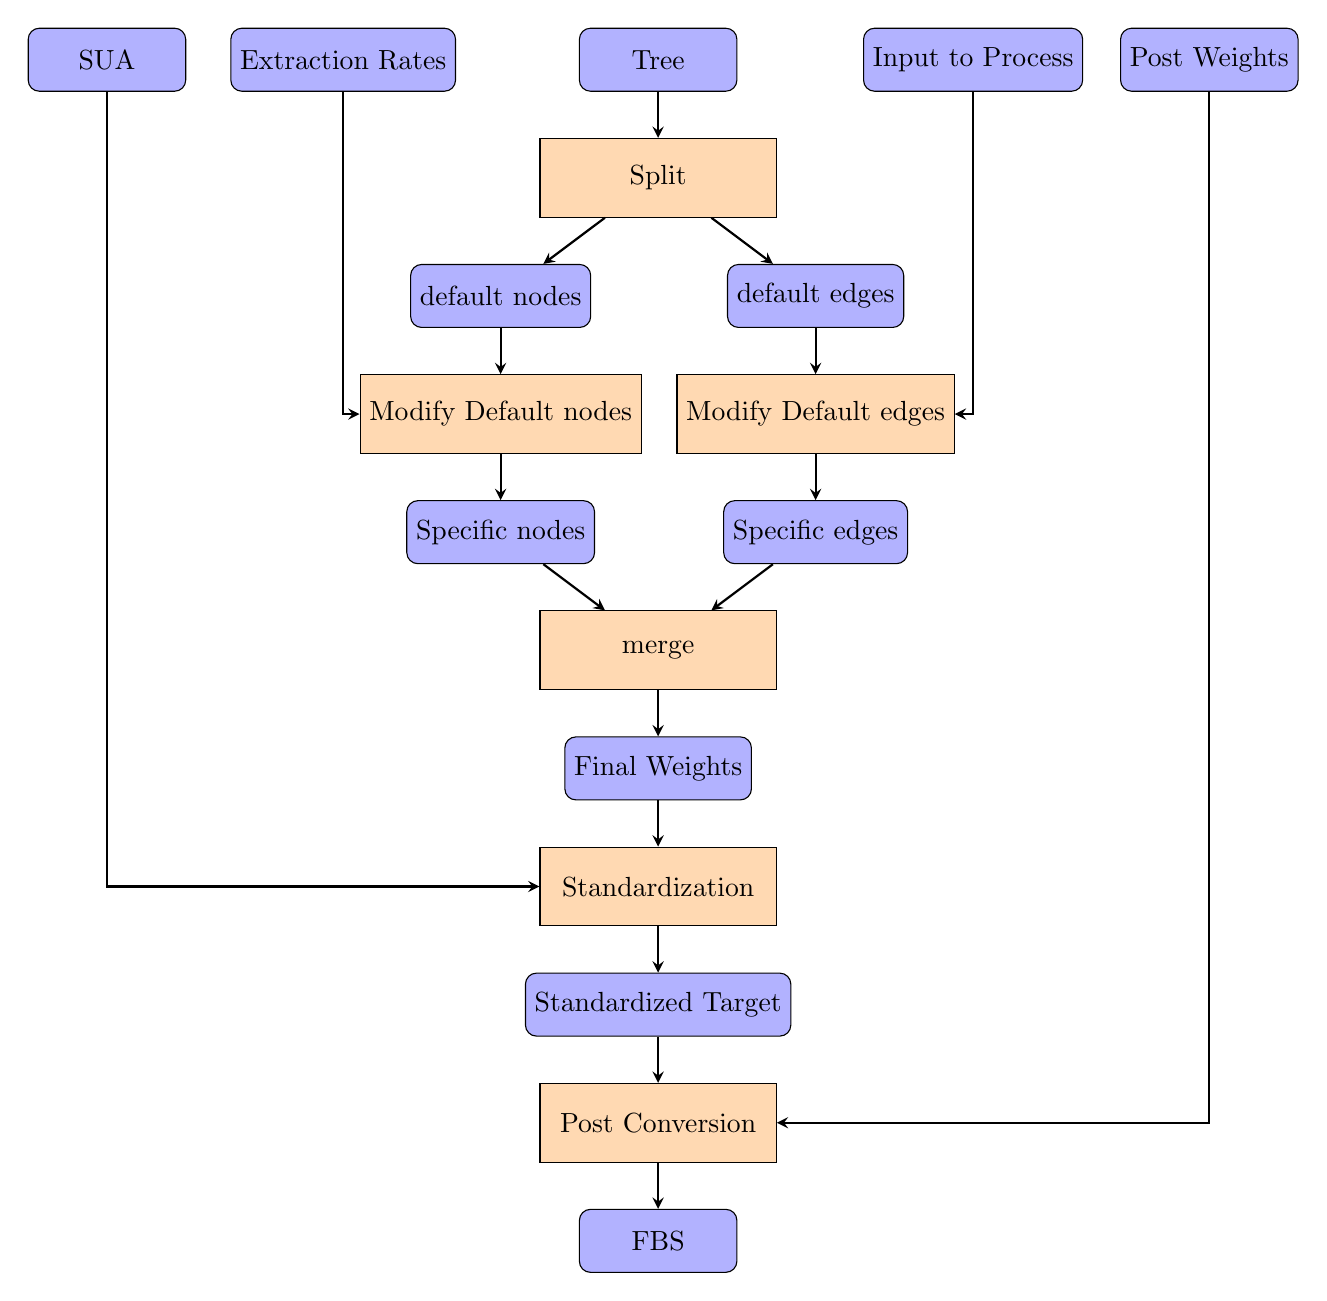
\begin{tikzpicture}[node distance=1.5cm]

%% nodes
\node (tree) [io, xshift=-2cm] {Tree};
\node (extract) [io, left of=tree, xshift=-2.5cm] {Extraction Rates};
\node (input) [io, right of=tree, xshift=2.5cm] {Input to Process};
\node (postWeights) [io, right of=input, xshift=1.5cm]{Post
  Weights};
\node (SUA) [io, left of=extract, xshift=-1.5cm]{SUA};
\node (split) [process, below of=tree]{Split};
\node (in2nodes) [io, below of=tree, xshift=-2cm, yshift=-1.5cm]
      {default nodes};
\node (in2edges) [io, below of=tree, xshift=2cm, yshift=-1.5cm]
      {default edges};
\node (in3nodes) [process, below of=in2nodes]{Modify Default nodes};
\node (in3edges) [process, below of=in2edges]{Modify Default edges};
\node (in4nodes) [io, below of=in3nodes]{Specific nodes};
\node (in4edges) [io, below of=in3edges]{Specific edges};
\node (merge) [process, below of=in4nodes, xshift=2cm]{merge};
\node (finalWeights) [io, below of=merge]{Final Weights};
\node (standardization) [process, below of=finalWeights]{Standardization};
\node (standardizedTarget) [io, below of=standardization]{Standardized
  Target};
\node (postConversion) [process, below of=standardizedTarget]{Post Conversion};
\node (FBS) [io, below of=postConversion]{FBS};


%% paths
\draw [arrow] (tree) -- (split);
\draw [arrow] (split) -- (in2nodes);
\draw [arrow] (split) -- (in2edges);
\draw [arrow] (in2nodes) -- (in3nodes);
\draw [arrow] (in2edges) -- (in3edges);
\draw [arrow] (extract) |- (in3nodes);
\draw [arrow] (input) |-  (in3edges);
\draw [arrow] (in3nodes) -- (in4nodes);
\draw [arrow] (in3edges) -- (in4edges);
\draw [arrow] (in4nodes) -- (merge);
\draw [arrow] (in4edges) -- (merge);
\draw [arrow] (merge) -- (finalWeights);
\draw [arrow] (finalWeights) -- (standardization);
\draw [arrow] (postWeights) |- (postConversion);
\draw [arrow] (SUA) |- (standardization);
\draw [arrow] (standardization) -- (standardizedTarget);
\draw [arrow] (standardizedTarget) -- (postConversion);
\draw [arrow] (postConversion) -- (FBS);

\end{tikzpicture}
\end{center}

In figure, the blue rectangle with rounded edges are data sets with
the elements at the top being the input data. The pink rectangles
boxes describe the procedures and steps to produce the final FBS. Each
pink rectangle box corresponds to an R function.



\subsection{Input Data set}

\subsubsection{SUA}

Here the SUA includes all the commodity which lies in the SUA domain,
and the elements of the Food Balance Sheet. That is, the elemenet 51
for production, 141 for food and etc.

\subsubsection{Extraction Rate}
This is dataset includes the same list of commodity except of the
primary commodity such as wheat. It is the extraction rate in which
process commodity such as wheat flour are multiplied in order to
obtain the wheat equivalent.

\subsubsection{Tree}
Currently, this list is taken from the old FBS system provided by
Rafik. It contains the default information how process commodity are
related to each other and their final fbs element. The file also
contains the default extraction rate to be applied to the commodity.

\subsubsection{Input to Process}

This data set is obtained from the "Input to Process" table from the
SUA, it contains information about how the old system calculates the
process commodity when it is not available.

\subsubsection{Post Weights}
This is list of weights to be multiplied at the end of the
standardization to obtain the final FBS elements. For example, rice
(27) is multiplied by 0.667 to obtain the rice and produce (2805) in
milled equivalent.


\subsection{Procedures}

\subsubsection{Split}
The first step is to split the data set \textbf{tree} into two
different piece of information. The nodes corresponds to information
about a certain commodity, such as whether they are a target commodity
and their default extraction rates. While the edge maps the
relationship of the commodities. Wheat flour to wheat, cheese to milk
so on and so forth.

\subsubsection{Modify default nodes}
In this step, the default extraction rates are modified when a country
and year specific extraction rates are available. In this case, the
specific rate replaces the default rate. The product to this process
is a country and year specific node table.

\subsubsection{Modify default edges}
Similar to the previous step, if there is a country specific tree as
indicated in the "input to process" data, then the specific tree is
taken. Further, the reverse share is calculated in this step. The
product is a country and year specific standardization path.

\subsubsection{Merge}
Finally, the nodes and edges are outer merged to include all possible
path and the direct weight is calculated. The direct weight is the
product of all the path to obtain a conversion number for highly
processed commodity such as bread to be converted back to its primary
equivalent.

%% \begin{equation}
$$
d_i = \prod_{i}^{p} (w_i \times 1/e_i)
$$
%% \end{equation}

Where the $w_t$ is the reverse weight, and $e_i$ is the extraction
rate.

\subsubsection{Standardization to Target}
After computing the direct weights, the standardization can be
performed by a simple multiplication followed by summation.

\subsubsection{Post Conversion}
Finally, the targets are multiplied by the post conversion factor to
obtain units in the final Food Balance Sheet. The list also contain
whether a target is included in the final FBS.







\end{document}
